\documentclass[oupdraft]{sysbio_sse}
%DIF LATEXDIFF DIFFERENCE FILE
%DIF DEL python-opentree_orig_sub.tex   Thu Apr  8 13:21:18 2021
%DIF ADD python-opentree.tex            Fri Apr 23 14:03:49 2021
%\usepackage[colorlinks=true, urlcolor=citecolor, linkcolor=citecolor, citecolor=citecolor]{hyperref}
\usepackage{url}
\usepackage{indentfirst}
\usepackage{color}
\usepackage{float}
%\usepackage{hyperref}
% Add history information for the article if required
%\history{Received Month X, 20XX;
%revised Month X, 20XX}
%\hypersetup{linkcolor=black, citecolor=black, colorlinks=true, hyperindex=true}
%DIF PREAMBLE EXTENSION ADDED BY LATEXDIFF
%DIF UNDERLINE PREAMBLE %DIF PREAMBLE
\RequirePackage[normalem]{ulem} %DIF PREAMBLE
\RequirePackage{color}\definecolor{RED}{rgb}{1,0,0}\definecolor{BLUE}{rgb}{0,0,1} %DIF PREAMBLE
\providecommand{\DIFadd}[1]{{\protect\color{blue}\uwave{#1}}} %DIF PREAMBLE
\providecommand{\DIFdel}[1]{{\protect\color{red}\sout{#1}}}                      %DIF PREAMBLE
%DIF SAFE PREAMBLE %DIF PREAMBLE
\providecommand{\DIFaddbegin}{} %DIF PREAMBLE
\providecommand{\DIFaddend}{} %DIF PREAMBLE
\providecommand{\DIFdelbegin}{} %DIF PREAMBLE
\providecommand{\DIFdelend}{} %DIF PREAMBLE
\providecommand{\DIFmodbegin}{} %DIF PREAMBLE
\providecommand{\DIFmodend}{} %DIF PREAMBLE
%DIF FLOATSAFE PREAMBLE %DIF PREAMBLE
\providecommand{\DIFaddFL}[1]{\DIFadd{#1}} %DIF PREAMBLE
\providecommand{\DIFdelFL}[1]{\DIFdel{#1}} %DIF PREAMBLE
\providecommand{\DIFaddbeginFL}{} %DIF PREAMBLE
\providecommand{\DIFaddendFL}{} %DIF PREAMBLE
\providecommand{\DIFdelbeginFL}{} %DIF PREAMBLE
\providecommand{\DIFdelendFL}{} %DIF PREAMBLE
%DIF LISTINGS PREAMBLE %DIF PREAMBLE
\RequirePackage{listings} %DIF PREAMBLE
\RequirePackage{color} %DIF PREAMBLE
\lstdefinelanguage{DIFcode}{ %DIF PREAMBLE
%DIF DIFCODE_UNDERLINE %DIF PREAMBLE
  moredelim=[il][\color{red}\sout]{\%DIF\ <\ }, %DIF PREAMBLE
  moredelim=[il][\color{blue}\uwave]{\%DIF\ >\ } %DIF PREAMBLE
} %DIF PREAMBLE
\lstdefinestyle{DIFverbatimstyle}{ %DIF PREAMBLE
	language=DIFcode, %DIF PREAMBLE
	basicstyle=\ttfamily, %DIF PREAMBLE
	columns=fullflexible, %DIF PREAMBLE
	keepspaces=true %DIF PREAMBLE
} %DIF PREAMBLE
\lstnewenvironment{DIFverbatim}{\lstset{style=DIFverbatimstyle}}{} %DIF PREAMBLE
\lstnewenvironment{DIFverbatim*}{\lstset{style=DIFverbatimstyle,showspaces=true}}{} %DIF PREAMBLE
%DIF END PREAMBLE EXTENSION ADDED BY LATEXDIFF

\begin{document}

% Title of paper
\title{OpenTree: A Python package for Accessing and Analyzing data from the Open Tree of Life}
% Each important word in the title should begin with a capital letter

% List of authors, with corresponding author marked by asterisk
\author{Emily Jane McTavish$^{1,\ast}$, Luna Luisa Sanchez Reyes$^{1}$, and
Mark T. Holder,$^{3}$\\[4pt]
% Author addresses
\textit{$^{1}$~Dept.~Life and Environmental Sciences, University of California, Merced, CA, USA 95343}
\\
\textit{$^{2}$~Dept.~Ecology and Evolutionary Biology, University of Kansas, Lawrence, KS USA 66045}\\
\textit{$^{3}$~Biodiversity Institute, University of Kansas, Lawrence, KS USA 66045}
\\[2pt]
% E-mail address for correspondence
\textit{*Corresponding author details here}}
% Identify the name, address, telephone/fax numbers, and e-mail address for the author who will receive proofs and be designated the "corresponding author" in text.

% Running headers of paper:
\markboth%
% First field is the short list of authors
{McTavish, Sanchez-Reyes, Holder}
% Second field is the short title of the paper
{opentree \DIFdelbegin \DIFdel{python }\DIFdelend \DIFaddbegin \DIFadd{Python }\DIFaddend package}
% This should be shortened version of the title and no greater than 50 characters

\maketitle

\begin{abstract}
{The Open Tree of Life project constructs a comprehensive, dynamic and digitally-available tree of life by synthesizing published phylogenetic trees along with taxonomic data.
Open Tree of Life provides web-service application programming interfaces (APIs) to make the tree estimate, unified taxonomy, and input phylogenetic data available to anyone.
Here, we describe the \DIFdelbegin \DIFdel{python }\DIFdelend \DIFaddbegin \DIFadd{Python }\DIFaddend package \texttt{opentree}, which provides a user friendly \DIFdelbegin \DIFdel{python }\DIFdelend \DIFaddbegin \DIFadd{Python }\DIFaddend wrapper for these APIs and a set of scripts and tutorials for straightforward downstream data analyses.
We demonstrate the utility of these tools by generating an estimate of the phylogenetic relationships of all bird families, and by capturing a phylogenetic estimate for all taxa  observed at the University of California Merced Vernal Pools and Grassland Reserve.
}

{Python, phylogenetics, taxonomy, evolution, open science.}
\end{abstract}
\newline

Evolutionary history provides a framework to link all life on earth. However, it is not easy to access accurate, up-to-date phylogenetic relationships for arbitrary sets of taxa of interest, even if phylogenetic estimates for those taxa have been made and published \citep{drew_lost_2013, mctavish_how_2017}. Individual phylogenetic estimates are not comprehensive, and therefore seldom contain all taxa of interest. Taxonomic relationships, while comprehensive, provide a coarse, and often outdated, picture of shared ancestry.
The Open Tree of Life project (OpenTree) provides a reproducible framework for accessing up-to-date \DIFaddbegin \DIFadd{and expert-knowledge-based }\DIFaddend evolutionary relationships for arbitrary sets of taxa across the entire tree of life.
All data in OpenTree is freely available via \DIFaddbegin \DIFadd{application programming interfaces (}\DIFaddend API's\DIFaddbegin \DIFadd{)}\DIFaddend .
The package \texttt{opentree} provides a user friendly \DIFdelbegin \DIFdel{python }\DIFdelend \DIFaddbegin \DIFadd{Python }\DIFaddend interface to access these data. In addition \texttt{opentree} is packaged with a set of tutorials and scripts to make common downstream analyses straightforward.

\bigskip
% Each important word in the heading level 1 should begin with a capital letter; no heading for the introduction
% Please note that the level 1 headings given here, e.g. Description, are suggestions only
\section{Description}
\label{sec2}

\texttt{opentree} is a Python package for accessing and analyzing data from the OpenTree of Life project.
Open Tree of Life stores a wealth of taxonomic and phylogenetic data gathered together in an open-access interoperable framework.
The current synthetic tree \citep{opentreeoflife_open_2019} comprises 2.4 million tips.
Most of the tips of the tree represent species, but some are infraspecific taxa.
The framework of this tree is provided by a unified taxonomy \citep{opentreeoflife_open_2019-1, rees_automated_2017}.
This taxonomy links unique identifiers across many online taxonomic resources, including NCBI \citep{federhen_ncbi_2012}, GBIF \citep{gbif_secretariat_gbif_2019}, as well as user contributed taxonomic amendments contained in [https://github.com/OpenTreeOfLife/amendments-1].
These taxonomic relationships are refined by evolutionary estimates from 1,216 published papers including 87,000 tip taxa \citep{opentreeoflife_open_2019, redelings_supertree_2017}.
The Open Tree data store, `Phylesystem' \citep{mctavish_phylesystem_2015} contains 4,500 published studies, including those incorporated in the \DIFdelbegin \DIFdel{tree. Each tree has mappings between the tips in these published studies and unique }\DIFdelend \DIFaddbegin \DIFadd{latest version of OpenTree's synthetic tree.
Phylogenies in the Phylesystem database have mappings between their tip names and unique OpenTree }\DIFaddend taxonomic identifiers.
\DIFaddbegin \DIFadd{There are several reasons trees are included in the `Phylesystem' data store but not the synthetic tree.
The complete curation of trees requires human intervention and confirmation at several steps, including vetting taxonomic name resolution service matches and correctly rooting trees, as many output files are shared as unrooted trees.
In addition, some of the trees in Phylesystem describe gene tree level or within species relationships, which are not appropriate for the species (and named subspecies) level relationships captured in the synthetic tree.
There is also lag between study upload, which makes studies immediately available via the API, and the time to re-build the entire synthetic tree, which is released in versioned increments (current version, 12.3)
The number of input studies increases in each successive synthesis tree release.
}\DIFaddend 

All of these data are freely accessible via API calls, documented at \url{https://github.com/OpenTreeOfLife/germinator/wiki/Open-Tree-of-Life-Web-APIs}.
\texttt{opentree} provides \DIFdelbegin \DIFdel{an }\DIFdelend \DIFaddbegin \DIFadd{a }\DIFaddend user-friendly wrapper for calling these APIs \DIFaddbegin \DIFadd{from the command line or in Python}\DIFaddend .
In addition, it converts these data between commonly used file formats and data types.
This package allows \DIFdelbegin \DIFdel{allows }\DIFdelend users to generate \DIFdelbegin \DIFdel{to data objects }\DIFdelend \DIFaddbegin \DIFadd{data objects to use }\DIFaddend in DendroPy, a \DIFaddbegin \DIFadd{widely cited Python }\DIFaddend phylogenetic computing library \citep{sukumaran_dendropy_2010}.


\texttt{opentree} incorporates in \DIFdelbegin \DIFdel{python }\DIFdelend \DIFaddbegin \DIFadd{Python }\DIFaddend the functionality available in rotl, an {R} package to interact with the Open Tree of Life data \citep{michonneau_rotl_2016}, as well as additional downstream analysis and interoperability tools.
\texttt{rotl} has been already been cited 132 times in the 4 years since its publication, demonstrating a demand for accessible user access to these data.
By providing a \DIFdelbegin \DIFdel{python }\DIFdelend \DIFaddbegin \DIFadd{Python }\DIFaddend package to interact with these data, we make it straightforward for \DIFdelbegin \DIFdel{python }\DIFdelend \DIFaddbegin \DIFadd{Python }\DIFaddend users to access and analyze these data.
A \DIFdelbegin \DIFdel{python }\DIFdelend \DIFaddbegin \DIFadd{Python }\DIFaddend wrapper for Open Tree of Life also makes linking these data with the stable of other Python biodiversity informatics tools straightforward.

\DIFdelbegin \DIFdel{In addition}\DIFdelend \DIFaddbegin \DIFadd{Finally}\DIFaddend , \texttt{opentree} expands the toolset available for working with \DIFdelbegin \DIFdel{the OpenTree}\DIFdelend \DIFaddbegin \DIFadd{OpenTree's }\DIFaddend unified taxonomy \citep{rees_automated_2017}.


\bigskip
\section{Services provided by opentree}
\label{sec3}


The OpenTree APIs are divided into three main categories\DIFdelbegin \DIFdel{, }\DIFdelend \DIFaddbegin \DIFadd{: }\DIFaddend synthetic tree, taxonomy and taxonomic name resolution, and study search.
Many analyses integrate calls to each of these subcomponents.
The \texttt{opentree} package links across these services to make common API calls easier.
Some example calls are described here, but all methods and scripts are fully documented, including examples and return formats at \url{https://opentree.readthedocs.io}.

\subsubsection{Synthetic tree.---} The OpenTree synthetic tree contains all 2.4 million taxa in the OpenTree taxonomy, with relationships for 87,000 taxa informed by 1,216 studies.
Each branch in the tree is informed by published phylogenetic relationships, where they are present in the curated data store, or by taxonomic relationships where no phylogenetic data is available.
For each node in the synthetic tree, the API returns identifiers for
all the \DIFdelbegin \DIFdel{trees }\DIFdelend \DIFaddbegin \DIFadd{phylogenies }\DIFaddend in the synthesis pipeline which support or conflict with that node.
Each node is uniquely labeled.
If the descendants of a node align with named taxonomic group, the taxon identifier is applied to the node.
If the node does not correspond \DIFaddbegin \DIFadd{to }\DIFaddend a taxon named in the OpenTree taxonomy, the node is labeled using a phyloreference \citep{parr_evolutionary_2012}\DIFdelbegin \DIFdel{describing }\DIFdelend \DIFaddbegin \DIFadd{, a unique name identifying }\DIFaddend that node as the most recent common ancestor of two \DIFdelbegin \DIFdel{identified }\DIFdelend \DIFaddbegin \DIFadd{named }\DIFaddend taxa.
\texttt{opentree} users can easily access evolutionary estimates for arbitrary sets of taxa.
The web-service response also includes the published \DIFdelbegin \DIFdel{phylogenetics }\DIFdelend \DIFaddbegin \DIFadd{phylogenetic }\DIFaddend estimates which underlie those inferences.
The \texttt{opentree} wrapper captures and formats these citations to make providing appropriate credit for these synthetic induced subtree estimates straightforward.
Users can also access full synthetic subtrees subtending any individual node.


\subsubsection{Taxonomy and Taxonomic Name Resolution.---} The OpenTree taxonomy not only provides a scaffold for the synthetic tree, but is also a valuable resource in its own right.
Matching names is a key hurdle in bioinformatics.
Correct taxon names change through time, and spelling and typographical errors can propagate through bioinformatic resources.
Thus, demanding exact matching of names from different sources can be too stringent and fail to match the same taxon.
However, different names can be very close in spelling to one another.
So, tolerating misspellings makes it easy to accidentally match names that should refer to two distinct taxa.
The OpenTree taxonomy \citep{rees_automated_2017, opentreeoflife_open_2019-1} provides a link between the unique identifiers generated by several large scale online taxonomic resources [GBIF, NCBI, Silva, Worms], as well as all known name synonomies provided by those resources.
The OpenTree taxonomic name resolution service (TNRS) searches this full taxonomy and returns exact or fuzzy matches from input names string to taxa and their unique \DIFaddbegin \DIFadd{taxonomic }\DIFaddend identifiers.
This TNRS forms a link between human readable name strings, and rigorous unique identifiers.

\texttt{opentree} wraps the OpenTree taxonomy and TNRS APIs for ease of integrating taxonomy and TNRS queries with downstream analyses. In addition, \texttt{opentree} provides helpers for quickly searching the text download of the taxonomy, which can be more efficient for bulk queries.


\subsubsection{Study search.---} The OpenTree datastore contains 4,468 published phylogenetic studies, including 9,395 \DIFdelbegin \DIFdel{phylogenetic trees }\DIFdelend \DIFaddbegin \DIFadd{phylogenies }\DIFaddend (as of Dec 4, 2020).
These studies and \DIFdelbegin \DIFdel{trees }\DIFdelend \DIFaddbegin \DIFadd{phylogenies }\DIFaddend are indexed on a number of properties including author name, curator name, and publication information.
In addition, the tips of these trees are mapped to the unified \DIFdelbegin \DIFdel{Open Tree }\DIFdelend \DIFaddbegin \DIFadd{OpenTree }\DIFaddend taxonomy making comparisons among estimates of relationships and searching for taxa of interest straightforward.
This allows searching of studies based on taxa contained in the study.
Importantly, this search does not rely on string-matching of what the taxonomic name was at the time of publication \DIFdelbegin \DIFdel{- rather}\DIFdelend \DIFaddbegin \DIFadd{-- rather, }\DIFaddend it leverages the full suite of synonomies gathered across the input taxonomies to find equivalent taxa across studies, even if the canonical name has changed between publications.
The indexing of these \DIFdelbegin \DIFdel{trees }\DIFdelend \DIFaddbegin \DIFadd{phylogenies }\DIFaddend is taxonomically explicit.
So, for example, a search for `canidae' will find \DIFdelbegin \DIFdel{trees }\DIFdelend \DIFaddbegin \DIFadd{phylogenies }\DIFaddend with taxa contained in the taxonomic group \DIFdelbegin \textit{\DIFdel{canidae}}%DIFAUXCMD
\DIFdelend \DIFaddbegin \DIFadd{Canidae}\DIFaddend , even if the term `canidae' does not itself appear in the \DIFdelbegin \DIFdel{tree }\DIFdelend \DIFaddbegin \DIFadd{phylogeny }\DIFaddend or tips.
Based on the results of these searches, studies can be viewed in a browser on the OpenTree curator site, or the phylogenies themselves can be downloaded for comparisons or other downstream use.

In addition, as the tips of each study are mapped by curators to \DIFaddbegin \DIFadd{taxonomic }\DIFaddend identifiers in the OpenTree taxonomy, comparing the relationships represented in input \DIFdelbegin \DIFdel{trees }\DIFdelend \DIFaddbegin \DIFadd{phylogenies }\DIFaddend to taxonomic relationships and to taxonomy is straightforward. The browser based tree viewer has a graphical visualization of this concordance and conflict. \texttt{opentree} provides a wrapper for this conflict functionality, which makes it straightforward to assess what taxon definitions and evolutionary relationships a \DIFdelbegin \DIFdel{tree }\DIFdelend \DIFaddbegin \DIFadd{phylogenetic }\DIFaddend estimate agrees with and conflicts with. This functionality can also be applied to local phylogenies for which the tips have been matched to taxonomy. This allows users to assess concordance and conflict with previous inferences in pre-publication \DIFdelbegin \DIFdel{trees}\DIFdelend \DIFaddbegin \DIFadd{phylogenies}\DIFaddend , even without sharing them to the publicly available OpenTree \DIFdelbegin \DIFdel{data store }\DIFdelend \DIFaddbegin \DIFadd{database }\DIFaddend \citep{reyes_physcraper_2020, mctavish_phylesystem_2015}.



\bigskip

\section{Biological Examples}
\label{sec4}

There are a plethora of downstream applications of this linked set of resources.
We highlight two examples based on user queries.


\subsection{A phylogeny of all bird families}
A full Jupyter notebook tutorial demonstrating how to access a \DIFaddbegin \DIFadd{synthetic }\DIFaddend tree of all bird families is packaged with the software at \url{https://github.com/OpenTreeOfLife/python-opentree/blob/main/docs/notebooks/TreeOfBirdGenera.ipynb}.
Capturing evolutionary information at large scales is often simplified by using arbitrary taxonomic cutoffs.
While the OpenTree taxonomy is not rank focused, it does track rank information from component taxonomies.
By searching the OpenTree taxonomy for families in birds, we find that there are 390 listed bird families, 196 of which are included in the synthetic tree.
Groups \DIFdelbegin \DIFdel{that }\DIFdelend are excluded from the synthetic tree for a few potential reasons, the most common of which is that all members of the group are extinct, and we have no curated published studies providing information about the correct evolutionary relationships.
Placements of fossil taxa based only on taxonomy tend to be unstable, and the OpenTree synthesis procedure excludes taxa if the taxon is not present in at least one  phylogenetic input.
These families can be included in later synthetic trees if \DIFdelbegin \DIFdel{data is }\DIFdelend \DIFaddbegin \DIFadd{new studies or phylogenies are }\DIFaddend added to the \DIFdelbegin \DIFdel{study corpus }\DIFdelend \DIFaddbegin \DIFadd{Phylesystem database, }\DIFaddend providing information on their relationships.
Other taxa are excluded from synthesis if issues have been raised about their taxonomic validity, such as if the name corresponds to a family that is `barren', i.e. it contains no species in the OpenTree taxonomy, or because the name was judged to be invalid by the OpenTree taxonomy merging software \citep{rees_automated_2017}.

If we request an induced subtree from \DIFdelbegin \DIFdel{the synthesis }\DIFdelend \DIFaddbegin \DIFadd{OpenTree's synthetic tree }\DIFaddend for these 164 taxa, we get back \DIFdelbegin \DIFdel{a tree }\DIFdelend \DIFaddbegin \DIFadd{an output subtree }\DIFaddend that has 150 tips. The return value also includes a list of non-monophyletic taxa.
Some of the non-monophyletic taxa map to internal nodes on our output \DIFdelbegin \DIFdel{tree}\DIFdelend \DIFaddbegin \DIFadd{subtree}\DIFaddend . In those cases, input phylogenies are telling us that these `families' are paraphyletic with respect to other families. Which studies contest the monophyly of a taxonomic clade can be easily accessed through the browser (e.g. https://tree.opentreeoflife.org/opentree/argus/ottol@603925) or via the \texttt{opentree} wrapper using queries to \texttt{opentree.synth\_subtree}. Figure \ref{birdfams} shows the \DIFdelbegin \DIFdel{shows the topology of the }\DIFdelend \DIFaddbegin \DIFadd{topology of }\DIFaddend 130 monophyletic bird families plus MRCA's of 20 additional non-monophyletic families as tips. The other 14 taxa are non-monophyletic families for which the MRCA is an internal node on the output \DIFdelbegin \DIFdel{tree}\DIFdelend \DIFaddbegin \DIFadd{subtree}\DIFaddend .


\begin{figure}[!h]
\centering\DIFdelbeginFL %DIFDELCMD < 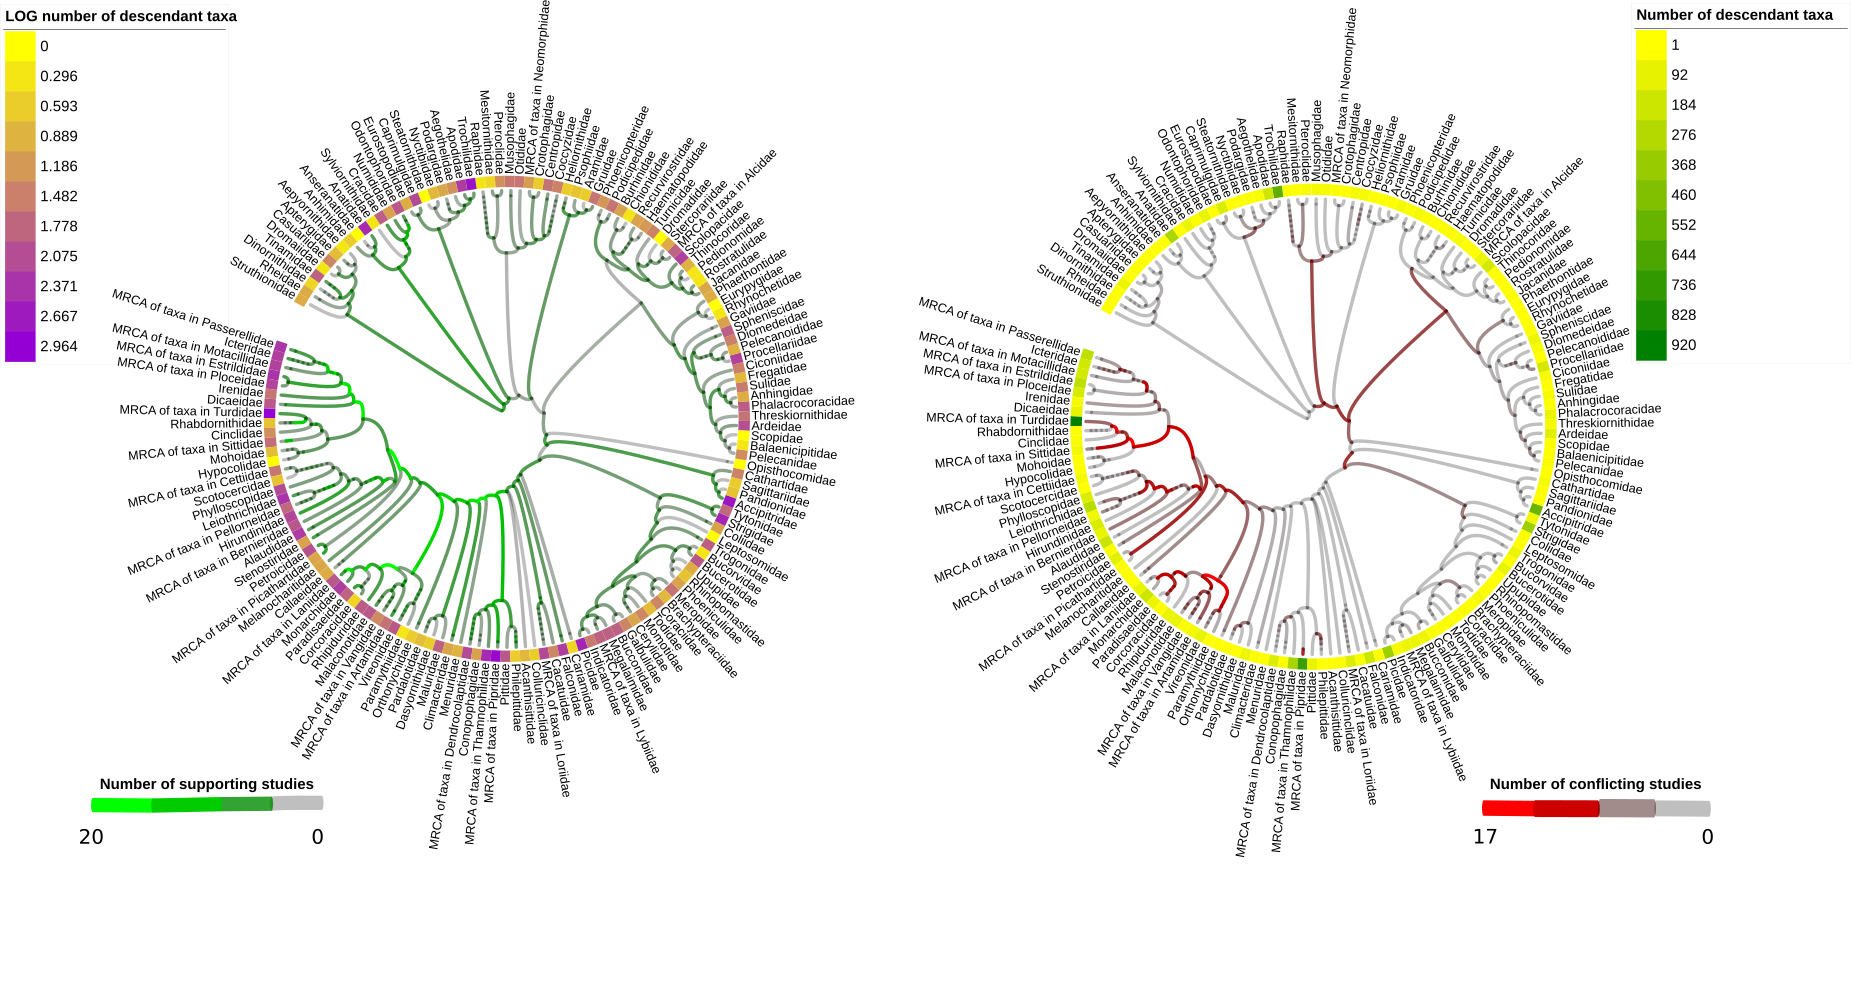
\includegraphics[width=\textwidth]{bird_fam_fig}
%DIFDELCMD < %%%
\DIFdelendFL \DIFaddbeginFL 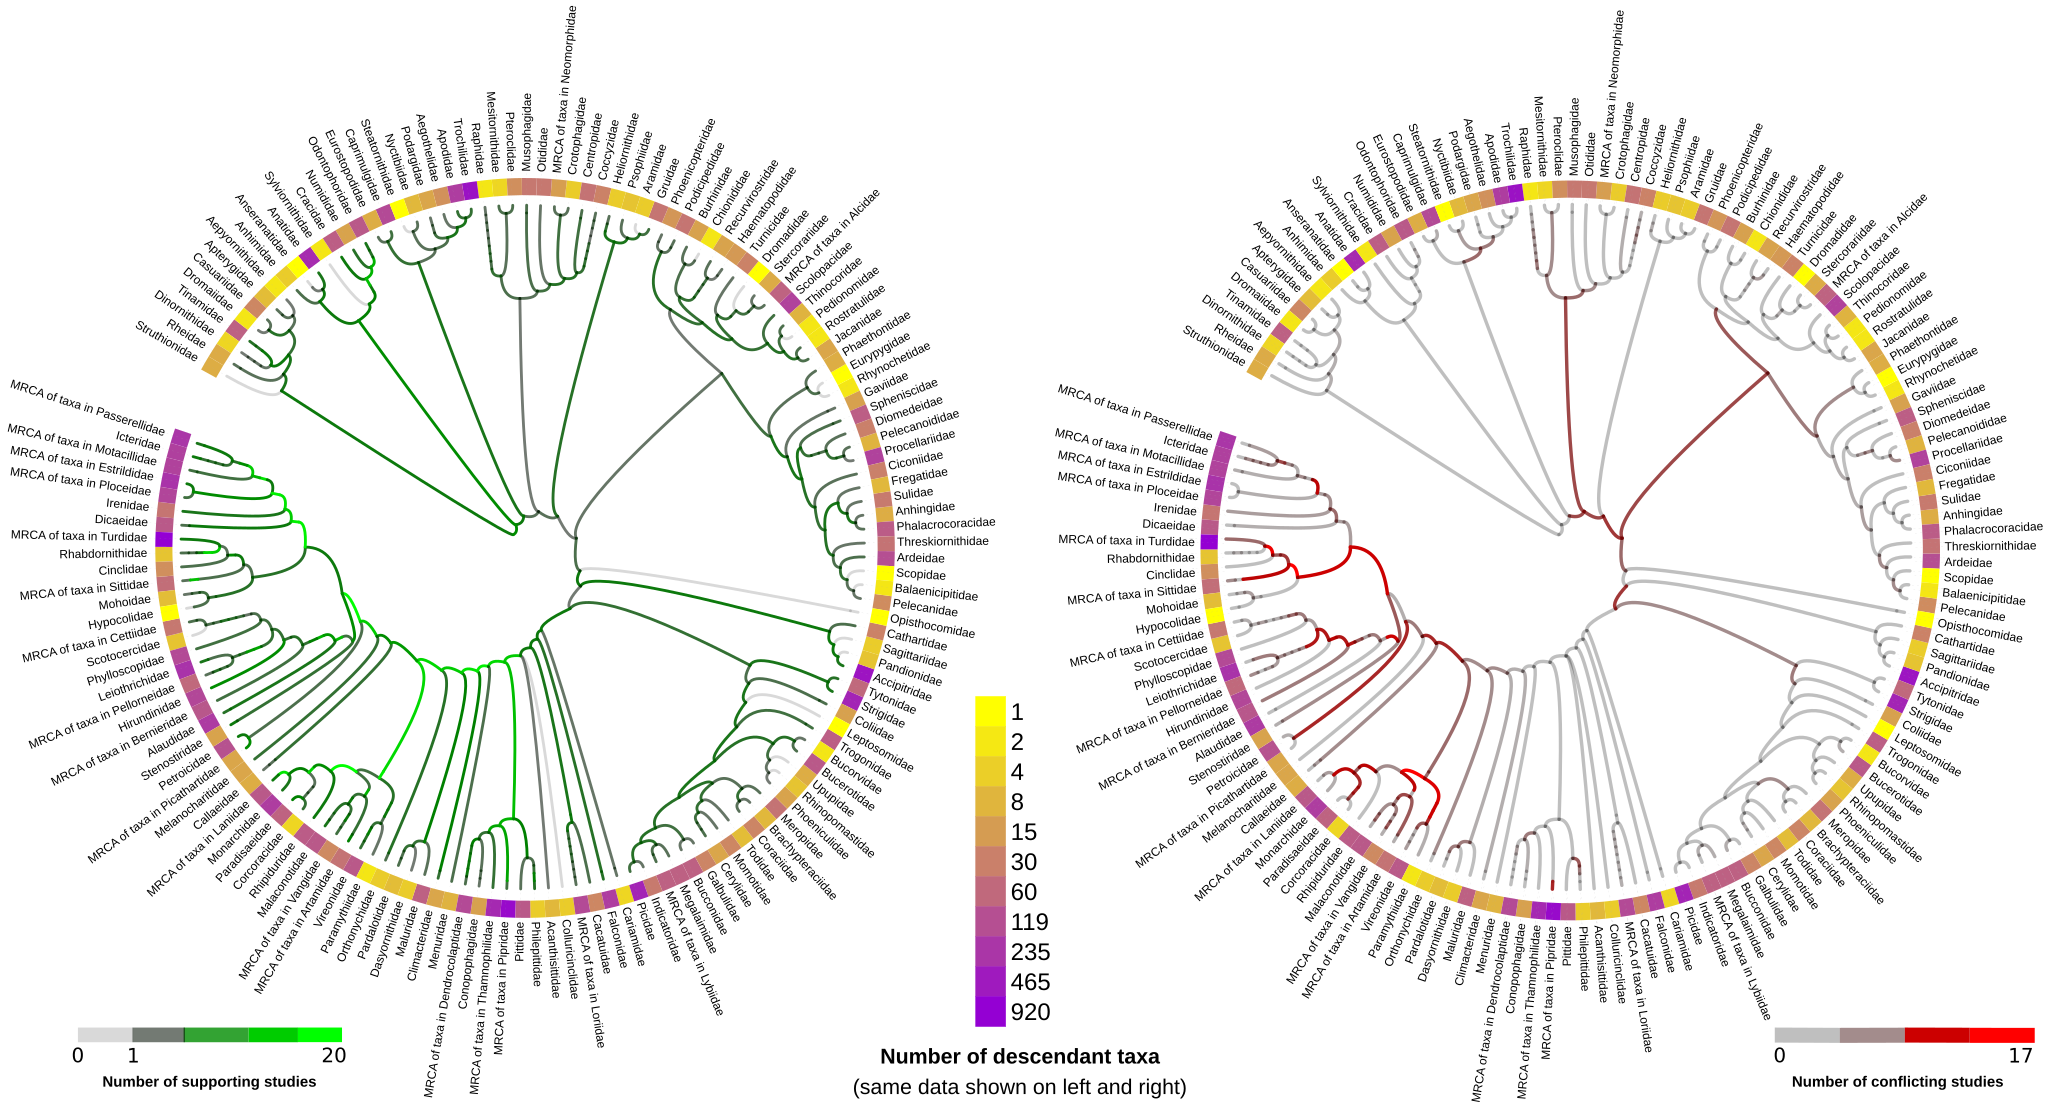
\includegraphics[width=\textwidth]{bird_fam_fig_rev}
\DIFaddendFL 

\caption{\DIFdelbeginFL \DIFdelFL{Relationships }\DIFdelendFL \DIFaddbeginFL \DIFaddFL{Phylogenetic relationships }\DIFaddendFL of 150 bird families \DIFdelbeginFL \DIFdelFL{, showing the number of published phylogenetic studies which support and and conflict with each branch in }\DIFdelendFL \DIFaddbeginFL \DIFaddFL{based on }\DIFaddendFL the \DIFaddbeginFL \DIFaddFL{latest OpenTree synthetic }\DIFaddendFL tree \DIFaddbeginFL \DIFaddFL{(v12.3)}\DIFaddendFL . For families which are not monophyletic according to published phylogenies, tips for those families are \DIFdelbeginFL \DIFdelFL{labelled }\DIFdelendFL \DIFaddbeginFL \DIFaddFL{labeled }\DIFaddendFL with 'MRCA of taxa in \DIFdelbeginFL \DIFdelFL{Family }\DIFdelendFL \DIFaddbeginFL \DIFaddFL{X family }\DIFaddendFL name'. Heat maps show the number of tip taxa descendants \DIFdelbeginFL \DIFdelFL{from }\DIFdelendFL \DIFaddbeginFL \DIFaddFL{in OpenTree within }\DIFaddendFL each tip\DIFdelbeginFL \DIFdelFL{, in log scale on left, and in exact numbers on left}\DIFdelendFL . Branch colors show the number of input studies which support (left, green) or conflict with (right, red) each inferred branch in the \DIFdelbeginFL \DIFdelFL{super }\DIFdelendFL \DIFaddbeginFL \DIFaddFL{synthetic }\DIFaddendFL tree. Branch lengths are arbitrary. A total of 64 published phylogenies underlie the relationships in this \DIFdelbeginFL \DIFdelFL{tree }\DIFdelendFL \DIFaddbeginFL \DIFaddFL{subtree }\DIFaddendFL (\DIFdelbeginFL \DIFdelFL{Citations }\DIFdelendFL \DIFaddbeginFL \DIFaddFL{citations }\DIFaddendFL in supplemental information). Figure created using \DIFaddbeginFL \DIFaddFL{the interactive Tree Of Life (iTOL) v4 }\DIFaddendFL \citep{letunic_interactive_2019}}
\label{birdfams}
\end{figure}

These families contain from 1 to 920 total descendant tip taxa (species and subspecies).
Across all 150 families, 10,357 \DIFdelbegin \DIFdel{descendent }\DIFdelend \DIFaddbegin \DIFadd{descendents }\DIFaddend tip taxa are captured by the relationships shown in this \DIFdelbegin \DIFdel{tree}\DIFdelend \DIFaddbegin \DIFadd{subtree}\DIFaddend .
Figure \ref{birdfams} displays the number of descendant taxa in each family as a heat map, with log of the number of descendants displayed on the left, and the actual number of \DIFdelbegin \DIFdel{descendents }\DIFdelend \DIFaddbegin \DIFadd{descendants }\DIFaddend on the right.
This display demonstrates that \DIFaddbegin \DIFadd{the use of }\DIFaddend `families' is not a very even way to break up biodiversity across birds.

\DIFdelbegin \DIFdel{Based on the }\DIFdelend \DIFaddbegin \DIFadd{Following OpenTree's }\DIFaddend phylogenetic synthesis algorithm \DIFaddbegin \DIFadd{\mbox{%DIFAUXCMD
\citep{redelings_supertree_2017}}\hspace{0pt}%DIFAUXCMD
}\DIFaddend , each branch in the \DIFaddbegin \DIFadd{synthetic }\DIFaddend tree is supported
by either taxonomy alone \DIFdelbegin \DIFdel{, }\DIFdelend \DIFaddbegin \DIFadd{(}\DIFaddend where there are no input \DIFaddbegin \DIFadd{phylogenetic }\DIFaddend studies that traverse that branch\DIFaddbegin \DIFadd{)}\DIFaddend , or by one or more input phylogenetic studies.
The \DIFaddbegin \DIFadd{source of }\DIFaddend support for each node in the \DIFaddbegin \DIFadd{synthetic }\DIFaddend tree can be interrogated using \DIFdelbegin \DIFdel{an }\DIFdelend \DIFaddbegin \DIFadd{a }\DIFaddend \texttt{\DIFdelbegin \DIFdel{opentree.}\DIFdelend synth\_node\_info\DIFdelbegin %DIFDELCMD < \MBLOCKRIGHTBRACE %%%
\DIFdel{call }\DIFdelend \DIFaddbegin } \DIFadd{function call from the }\texttt{\DIFadd{OpenTree}} \DIFadd{class in the package here presented}\DIFaddend .
While each branch must be supported by taxonomy or at least one input study from \DIFdelbegin \DIFdel{phylesystem}\DIFdelend \DIFaddbegin \DIFadd{Phylesystem}\DIFaddend , where multiple inputs traverse a branch, there can be conflict among studies.
\DIFdelbegin \DIFdel{The }\DIFdelend \DIFaddbegin \DIFadd{OpenTree's }\DIFaddend synthesis algorithm is greedy, and the \DIFdelbegin \DIFdel{output }\DIFdelend \DIFaddbegin \DIFadd{synthetic }\DIFaddend tree will display the branch supported by the highest ranked study included in synthesis.
The \DIFdelbegin \DIFdel{node info call }\DIFdelend \DIFaddbegin \texttt{\DIFadd{synth\_node\_info}} \DIFadd{function }\DIFaddend will return not only which studies support \DIFdelbegin \DIFdel{that }\DIFdelend \DIFaddbegin \DIFadd{any }\DIFaddend branch, but also which studies have relationships which conflict with that branch.
In figure \ref{birdfams}\DIFaddbegin \DIFadd{, }\DIFaddend support or conflict for each branch is displayed by the intensity of green and red coloration, respectively. Some branches in this \DIFdelbegin \DIFdel{tree }\DIFdelend \DIFaddbegin \DIFadd{subtree }\DIFaddend are supported by 20 studies, and a few show conflict with up to 17 other studies. Of the 443 branches in this \DIFdelbegin \DIFdel{tree}\DIFdelend \DIFaddbegin \DIFadd{subtree}\DIFaddend , 422 are supported by at least one input phylogenetic study, and the other 21 are based on taxonomic relationships.

\DIFdelbegin \DIFdel{This }\DIFdelend \DIFaddbegin \DIFadd{It is important to note that OpenTree's synthetic }\DIFaddend tree shows only topology. When combining taxonomy, and phylogenetic branches from across studies with vastly different data types, merging branch lengths is not meaningful. \DIFdelbegin \DIFdel{However, estimates of node ages can be gathered using downstream tools such as DateLife \mbox{%DIFAUXCMD
\citep{sanchez-reyes_datelife_2019} }\hspace{0pt}%DIFAUXCMD
which gathers and synthesizes node date information from studies  in the phylesystem corpus}\DIFdelend \DIFaddbegin \DIFadd{For downstream analyses requiring branch lengths, users have scaled topologies inferred from OpenTree using a variety of data types and rate-smoothing approaches e.g. \mbox{%DIFAUXCMD
\citep{smith2018constructing, smith2019pyphlawd, eastman2013congruification, allen2019spatial, li2019common, uyeda2017evolution, geffroy2020evolutionary, jantzen2019effects, sanchez-reyes_datelife_2019}}\hspace{0pt}%DIFAUXCMD
}\DIFaddend .

\subsection{Linking data from the Global Biodiversity Information Facility (GBIF) with phylogenetic information from Open Tree of Life}

\bigskip

The University of California \DIFaddbegin \DIFadd{(UC)}\DIFaddend , Merced has a natural reserve directly adjacent to campus, which contains several vernal pools. These vernal pools create a unique habitat which allows native species to thrive, and the proximity to campus allows undergraduate classes to experience this ecosystem on field trips which can be accomplished during class time.
A species list for the reserve and adjacent campus areas is available through \DIFaddbegin \DIFadd{the }\DIFaddend Global Biodiversity Information Facility (GBIF) website \citep{gbif_secretariat_gbif_2019}. GBIF provides a repository for species occurrence data tracked in a variety of data stores, including bird observations from eBird \citep{sullivan_ebird_2009}, community science observations from iNaturalist (\url{www.inaturalist.org}), and several other resources. A full tutorial demonstrating how to access a \DIFdelbegin \DIFdel{tree }\DIFdelend \DIFaddbegin \DIFadd{subtree }\DIFaddend for a GBIF data download is \DIFdelbegin \DIFdel{packaged with the software }\DIFdelend \DIFaddbegin \DIFadd{included with this package }\DIFaddend at \url{https://github.com/OpenTreeOfLife/python-opentree/blob/main/docs/notebooks/gbif/GBIF_to_OpenTree.ipynb}.

We downloaded the full list of animal observations from the UC Merced Vernal pools reserve from GBIF \citep{gbif_secretariat_gbif_2019}. This data download comprised 6,709 records from 223 species. Using the GBIF unique taxon identifiers, 201 of these species could be directly matched to taxa in the OpenTree taxonomy using \texttt{opentree.taxon\_info(source\_id = {gbif unique identifier})}. This direct matching captures exact one to one relationships between these taxonomies, and avoids slow and potentially error prone string matching. Nineteen taxa had updated identifiers in GBIF since the most recent reconciliation between the GBIF taxonomy and the OpenTree taxonomy, and were assigned OpenTree taxon identifiers based on exact string matches. There were two taxa ``\textit{P. abortivum} St.'' and ``\textit{Ichneumon cupitus} Cresson 1877'', which were not found in the OpenTree taxonomy, and were dropped from the analysis.


Using this set of 223 OpenTree unique identifiers, an induced synthetic tree for these taxa can be downloaded (Figure \ref{vernalanimals}). This synthetic tree is supported by 160 individual published trees (\DIFdelbegin \DIFdel{Citations }\DIFdelend \DIFaddbegin \DIFadd{citations }\DIFaddend in supplemental information)\DIFdelbegin \DIFdel{)}\DIFdelend .

\begin{figure}[!h]
\centering
\includegraphics[width=\textwidth]{vernal_animals}
\caption{Evolutionary relationships between all animal taxon records in the UC Merced Vernal Pools and Grassland Reserve. Branch lengths are arbitrary. A total of 160 published phylogenies underlie the relationships in this tree (\DIFdelbeginFL \DIFdelFL{Citations }\DIFdelendFL \DIFaddbeginFL \DIFaddFL{citations }\DIFaddendFL in supplemental information). Figure created using \citep{letunic_interactive_2019}}
\label{vernalanimals}
\end{figure}



For researchers, working in the vernal pools reserve, this \DIFdelbegin \DIFdel{tree }\DIFdelend \DIFaddbegin \DIFadd{subtree }\DIFaddend also provides the necessary information for community phylogenetic analyses. \citet{li_for_2019} demonstrated that synthetic phylogenies from the OpenTree project perform well in community phylogenetic studies. By providing ready access to these estimates, based on 160 previously published \DIFdelbegin \DIFdel{trees}\DIFdelend \DIFaddbegin \DIFadd{phylogenies}\DIFaddend , \texttt{opentree} makes basing ecological analyses in an accurate evolutionary framework straightforward.


The ability to build a phylogeny of local taxa is also a valuable pedagogical tool. One of us (EJM) used this phylogeny to discuss the diversity of life of animal life as part of a class exercise on vernal pools ecology and evolution, in an undergraduate evolution class.
Students visited the UC Merced Vernal Pools and Grassland Reserve, and then explored the evolutionary \DIFdelbegin \DIFdel{tree }\DIFdelend \DIFaddbegin \DIFadd{relationships }\DIFaddend of all the animal species recorded as observed in the reserve.
There are several threatened and endangered species on the vernal pools reserve, including two species of fairy shrimp, \textit{Branchinecta lynchii} (threatened) and \textit{Branchinecta mesovallensis} (endangered).
By \DIFdelbegin \DIFdel{building a phylogenetic tree }\DIFdelend \DIFaddbegin \DIFadd{working with a subtree }\DIFaddend of taxa found on and around campus, tree thinking examples in class can have a direct connection for students. For example, this \DIFdelbegin \DIFdel{tree }\DIFdelend \DIFaddbegin \DIFadd{subtree }\DIFaddend (Figure \ref{vernalanimals}) shows that the genus \DIFaddbegin \DIFadd{of dabbling ducks, }\DIFaddend \textit{Anas}\DIFaddbegin \DIFadd{, }\DIFaddend does not form a monophyletic group. Walking the tree of life has been demonstrated to be an effective way to get students to understand the connections among different lineages of life on earth \citep{ballen_walking_2017}. Walking through this \DIFdelbegin \DIFdel{tree, and labelling }\DIFdelend \DIFaddbegin \DIFadd{subtree, and labeling }\DIFaddend major animal groups allows students to connect to the diversity of animal life based on the actual species surrounding them, rather than arbitrary textbook examples.

\DIFaddbegin \bigskip
\DIFaddend \section{\DIFdelbegin \DIFdel{Availability}\DIFdelend \DIFaddbegin \DIFadd{Discussion}\DIFaddend }
\label{sec5}

\DIFaddbegin \DIFadd{The OpenTree project makes available a synthetic tree across 2.4 million taxa, as well as thousands of peer-reviewed and published phylogenies that together can be reused for applications
from scientific discovery to education, conservation and
outreach \mbox{%DIFAUXCMD
\citep{stoltzfus2013phylotastic, mctavish_phylesystem_2015, rosindell2012onezoom, wong2020dynamic}}\hspace{0pt}%DIFAUXCMD
.
While several tools can generate phylogenies from DNA sequence data mined from the GenBank genetic database e.g. \mbox{%DIFAUXCMD
\citep{smith2009mega, sanderson2008phylota, antonelli2014supersmart, reyes_physcraper_2020}}\hspace{0pt}%DIFAUXCMD
, for regions of the tree where phylogenetic estimates already exist, relying on published peer-reviewed inferences of relationships is more efficient and accurate than generating new estimates \mbox{%DIFAUXCMD
\citep{smith2018constructing, owen2015synthetic, brown2017development, ewers2019towards}}\hspace{0pt}%DIFAUXCMD
.
Broad taxon sampling coverage is key to correctly estimate phylogenetic
diversity \mbox{%DIFAUXCMD
\citep{jantzen2019effects, park2018taxon}}\hspace{0pt}%DIFAUXCMD
, and genetic data is usually not available for all taxa in a community or a biological group of study.
}

\DIFadd{Many researchers have applied the OpenTree synthetic tree and data stores to answering their research questions across the breadth of both the tree of life, and the breadth of biological research domains.
In contrast to existing phylogenetic data stores, \mbox{%DIFAUXCMD
\citep{piel2000treebase}}\hspace{0pt}%DIFAUXCMD
, the links across studies provided by OpenTree and the synthesis algorithm make it possible to extract inferences for an arbitrary subset of taxa, and combine inferences from trees with few or no overlapping tips.
Several studies have used OpenTree resources to consolidate evolutionary estimates across a taxon (freshwater crayfish \mbox{%DIFAUXCMD
\citep{owen2015synthetic}}\hspace{0pt}%DIFAUXCMD
; birds \mbox{%DIFAUXCMD
\citep{brown2017development}}\hspace{0pt}%DIFAUXCMD
; barnacles \mbox{%DIFAUXCMD
\citep{ewers2019towards, ewers2019testing}}\hspace{0pt}%DIFAUXCMD
, mammals \mbox{%DIFAUXCMD
\citep{uyeda2017evolution}}\hspace{0pt}%DIFAUXCMD
).
Large scale synthetic phylogenies provide the opportunity to study the evolution and phylogenetic distribution of life history traits at large scales  \mbox{%DIFAUXCMD
\citep{tarka2018sex, healy2019animal, capdevila2020longevity}}\hspace{0pt}%DIFAUXCMD
.
Other trait evolution anayses on OpenTree synthesis subtrees include antipredator behavior associations with human interactions, \mbox{%DIFAUXCMD
\citep{geffroy2020evolutionary}}\hspace{0pt}%DIFAUXCMD
, effects of anthropogenic noise on
animal behavior  \mbox{%DIFAUXCMD
\citep{kunc2019effects}}\hspace{0pt}%DIFAUXCMD
, phylogenetic patterns of global wildlife trade,  \mbox{%DIFAUXCMD
\citep{fukushima2020global}}\hspace{0pt}%DIFAUXCMD
,  miniaturization in insects \mbox{%DIFAUXCMD
\citep{polilov2017scaling}}\hspace{0pt}%DIFAUXCMD
,
shoot flammability evolution \mbox{%DIFAUXCMD
\citep{cui2020shoot}}\hspace{0pt}%DIFAUXCMD
, and host symbiont dependence \mbox{%DIFAUXCMD
\citep{fisher2017evolution}}\hspace{0pt}%DIFAUXCMD
. 
OpenTree's synthetic tree provides a phylogentic backbone for commuity phylpogenetics analyses \mbox{%DIFAUXCMD
\citep{li2019common, jantzen2019effects}}\hspace{0pt}%DIFAUXCMD
.
In molecular biology, \mbox{%DIFAUXCMD
\citep{boeckmann2015quest} }\hspace{0pt}%DIFAUXCMD
used a phylogentic estimate across prokaryotes and eukaryotes to understand the evolution
of gene families and taxa to improve orthology prediction for phylogenetic applications.
\mbox{%DIFAUXCMD
\citep{herrera2015predicting} }\hspace{0pt}%DIFAUXCMD
used an OpenTree's synthetic subtree to predict RAD-seq marker cleavage site numbers
across the eukaryotic tree of life to guide the design of genome-wide genotypic and
sequencing projects.
\mbox{%DIFAUXCMD
\citep{miller2020codonpairs} }\hspace{0pt}%DIFAUXCMD
found that codon pairing biases are conserved across the diversity and can  be used for phylogenomic analyses.
}


\DIFadd{This }\texttt{\DIFadd{opentree}} \DIFadd{python toolkit expands user access to the OpenTree API's, and provides tutorials on how to easily access up to date evolutionary information across the entire tree of life, which will continue to facilitate biological research and outreach.
}


\section{\DIFadd{Availability}}
\label{sec6}

\DIFaddend \texttt{opentree} is fully open source with a CC0 license. It is available on GitHub \url{ https://github.com/OpenTreeOfLife/python-opentree}. It can be installed from PyPi using \texttt{pip install opentree}. The code is packaged with an automated test suite which is maintained to cover at minimum 75\% of the code. Testing reports are generated on \url{travis.io} and posted to {codecov.io} and reflected on the GitHub readme with each commit. Documentation and tutorials are available with the code, and \DIFdelbegin \DIFdel{is }\DIFdelend \DIFaddbegin \DIFadd{are }\DIFaddend posted to \url{https://opentree.readthedocs.io}.


\section{Conflict of Interest}
None

\section{Funding}
Funding for this project was provided by NSF ABI 1759846 and NSF ABI 1759838.

%If you have any acknowledgements, please include them here.
\section{\DIFdelbegin \DIFdel{Acknowledgements}\DIFdelend \DIFaddbegin \DIFadd{Acknowledgments}\DIFaddend }
This package relies on the OpenTree API's and the team that continues to develop and improve them, currently Jim Allman, Karen Cranston, Ben Redelings, and the authors of this package. We acknowledge logistical support provided by the UC Merced Vernal Pools and Grassland Reserve.
Thank you to Emily Sessa and the organizers of the Society of Systematic Biologists SSB 2020 meeting for supporting the workshop where we tested and demonstrated this package.

%If your paper has accompanying supplementary data, please include the below statement in your PDF.
%\section{Supplementary Material}
%Data available from the Dryad Digital Repository:
% \href{http://dx.doi.org/10.5061/dryad.[NNNN]}%
% {http://dx.doi.org/10.5061/dryad.[NNNN]}.
%\url{http://dx.doi.org/10.5061/dryad.[NNNN]}.

\bigskip\bigskip

%%%%%%%%%%%%%%%%%%%% REFERENCES %%%%%%%%%%%%%%%%%%
\DIFdelbegin %DIFDELCMD < 

%DIFDELCMD < %%%
%DIF <  The best way to enter references is to use BibTeX.
\DIFdelend \bibliographystyle{plainnat}
\DIFdelbegin %DIFDELCMD < \begin{thebibliography}{18}
%DIFDELCMD < \providecommand{\natexlab}[1]{#1}
%DIFDELCMD < \providecommand{\url}[1]{\texttt{#1}}
%DIFDELCMD < \expandafter\ifx\csname %%%
\DIFdel{urlstyle}%DIFDELCMD < \endcsname\relax
%DIFDELCMD <   \providecommand{\doi}[1]{doi: #1}\else
%DIFDELCMD <   \providecommand{\doi}{doi: \begingroup \urlstyle{rm}\Url}\fi
%DIFDELCMD < 

%DIFDELCMD < \bibitem[Ballen and Greene(2017)]{ballen_walking_2017}
%DIFDELCMD < %%%
\DIFdel{Cissy~J. Ballen and Harry~W. Greene.
}%DIFDELCMD < \newblock %%%
\DIFdel{Walking and talking the tree of life: }%DIFDELCMD < {%%%
\DIFdel{Why}%DIFDELCMD < } %%%
\DIFdel{and how to teach about
  biodiversity.
}%DIFDELCMD < \newblock %%%
\emph{\DIFdel{PLOS Biology}}%DIFAUXCMD
\DIFdel{, 15}%DIFDELCMD < \penalty0 %%%
\DIFdel{(3):}%DIFDELCMD < \penalty0 %%%
\DIFdel{e2001630, March 2017.
}%DIFDELCMD < \newblock %%%
\DIFdel{ISSN 1545-7885.
}%DIFDELCMD < \newblock \doi{10.1371/journal.pbio.2001630}%%%
\DIFdel{.
}%DIFDELCMD < \newblock %%%
\DIFdel{URL
  }%DIFDELCMD < \url{https://journals.plos.org/plosbiology/article?id=10.1371/journal.pbio.2001630}%%%
\DIFdel{.
}%DIFDELCMD < \newblock %%%
\DIFdel{Publisher: Public Library of Science.
}%DIFDELCMD < 

%DIFDELCMD < \bibitem[Drew et~al.(2013)Drew, Gazis, Cabezas, Swithers, Deng, Rodriguez,
%DIFDELCMD <   Katz, Crandall, Hibbett, and Soltis]{drew_lost_2013}
%DIFDELCMD < %%%
\DIFdel{Bryan~T. Drew, Romina Gazis, Patricia Cabezas, Kristen~S. Swithers, Jiabin
  Deng, Roseana Rodriguez, Laura~A. Katz, Keith~A. Crandall, David~S. Hibbett,
  and Douglas~E. Soltis.
}%DIFDELCMD < \newblock %%%
\DIFdel{Lost branches on the tree of life.
}%DIFDELCMD < \newblock %%%
\emph{\DIFdel{PLOS Biol}}%DIFAUXCMD
\DIFdel{, 11}%DIFDELCMD < \penalty0 %%%
\DIFdel{(9):}%DIFDELCMD < \penalty0 %%%
\DIFdel{e1001636, September 2013.
}%DIFDELCMD < \newblock %%%
\DIFdel{ISSN 1545-7885.
}%DIFDELCMD < \newblock \doi{10.1371/journal.pbio.1001636}%%%
\DIFdel{.
}%DIFDELCMD < \newblock %%%
\DIFdel{URL
  }%DIFDELCMD < \url{http://journals.plos.org/plosbiology/article?id=10.1371/journal.pbio.1001636}%%%
\DIFdel{.
}%DIFDELCMD < \newblock %%%
\DIFdel{Number: 9.
}%DIFDELCMD < 

%DIFDELCMD < \bibitem[Federhen(2012)]{federhen_ncbi_2012}
%DIFDELCMD < %%%
\DIFdel{Scott Federhen.
}%DIFDELCMD < \newblock %%%
\DIFdel{The }%DIFDELCMD < {%%%
\DIFdel{NCBI}%DIFDELCMD < } {%%%
\DIFdel{Taxonomy}%DIFDELCMD < } %%%
\DIFdel{database.
}%DIFDELCMD < \newblock %%%
\emph{\DIFdel{Nucleic Acids Research}}%DIFAUXCMD
\DIFdel{, 40}%DIFDELCMD < \penalty0 %%%
\DIFdel{(D1):}%DIFDELCMD < \penalty0 %%%
\DIFdel{D136--D143,
  January 2012.
}%DIFDELCMD < \newblock %%%
\DIFdel{ISSN 0305-1048.
}%DIFDELCMD < \newblock \doi{10.1093/nar/gkr1178}%%%
\DIFdel{.
}%DIFDELCMD < \newblock %%%
\DIFdel{URL }%DIFDELCMD < \url{https://academic.oup.com/nar/article/40/D1/D136/2903327}%%%
\DIFdel{.
}%DIFDELCMD < \newblock %%%
\DIFdel{Publisher: Oxford Academic.
}%DIFDELCMD < 

%DIFDELCMD < \bibitem[Letunic and Bork(2019)]{letunic_interactive_2019}
%DIFDELCMD < %%%
\DIFdel{Ivica Letunic and Peer Bork.
}%DIFDELCMD < \newblock %%%
\DIFdel{Interactive }%DIFDELCMD < {%%%
\DIFdel{Tree}%DIFDELCMD < } {%%%
\DIFdel{Of}%DIFDELCMD < } {%%%
\DIFdel{Life}%DIFDELCMD < } %%%
\DIFdel{(}%DIFDELCMD < {%%%
\DIFdel{iTOL}%DIFDELCMD < }%%%
\DIFdel{) v4: recent updates and new
  developments.
}%DIFDELCMD < \newblock %%%
\emph{\DIFdel{Nucleic Acids Research}}%DIFAUXCMD
\DIFdel{, 47}%DIFDELCMD < \penalty0 %%%
\DIFdel{(W1):}%DIFDELCMD < \penalty0 %%%
\DIFdel{W256--W259,
  July 2019.
}%DIFDELCMD < \newblock %%%
\DIFdel{ISSN 0305-1048.
}%DIFDELCMD < \newblock \doi{10.1093/nar/gkz239}%%%
\DIFdel{.
}%DIFDELCMD < \newblock %%%
\DIFdel{URL }%DIFDELCMD < \url{https://academic.oup.com/nar/article/47/W1/W256/5424068}%%%
\DIFdel{.
}%DIFDELCMD < \newblock %%%
\DIFdel{Publisher: Oxford Academic.
}%DIFDELCMD < 

%DIFDELCMD < \bibitem[Li et~al.(2019)Li, Trotta, Marx, Allen, Sun, Soltis, Soltis,
%DIFDELCMD <   Guralnick, and Baiser]{li_for_2019}
%DIFDELCMD < %%%
\DIFdel{Daijiang Li, Lauren Trotta, Hannah~E. Marx, Julie~M. Allen, Miao Sun,
  Douglas~E. Soltis, Pamela~S. Soltis, Robert~P. Guralnick, and Benjamin
  Baiser.
}%DIFDELCMD < \newblock %%%
\DIFdel{For common community phylogenetic analyses, go ahead and use
  synthesis phylogenies.
}%DIFDELCMD < \newblock %%%
\emph{\DIFdel{Ecology}}%DIFAUXCMD
\DIFdel{, 100}%DIFDELCMD < \penalty0 %%%
\DIFdel{(9):}%DIFDELCMD < \penalty0 %%%
\DIFdel{e02788, 2019.
}%DIFDELCMD < \newblock %%%
\DIFdel{ISSN 1939-9170.
}%DIFDELCMD < \newblock \doi{https://doi.org/10.1002/ecy.2788}%%%
\DIFdel{.
}%DIFDELCMD < \newblock %%%
\DIFdel{URL
  }%DIFDELCMD < \url{https://esajournals.onlinelibrary.wiley.com/doi/abs/10.1002/ecy.2788}%%%
\DIFdel{.
}%DIFDELCMD < \newblock %%%
\DIFdel{\_eprint:
  https://esajournals.onlinelibrary.wiley.com/doi/pdf/10.1002/ecy.2788.
}%DIFDELCMD < 

%DIFDELCMD < \bibitem[McTavish et~al.(2015)McTavish, Hinchliff, Allman, Brown, Cranston,
%DIFDELCMD <   Holder, Rees, and Smith]{mctavish_phylesystem_2015}
%DIFDELCMD < %%%
\DIFdel{Emily~Jane McTavish, Cody~E. Hinchliff, James~F. Allman, Joseph~W. Brown,
  Karen~A. Cranston, Mark~T. Holder, Jonathan~A. Rees, and Stephen~A. Smith.
}%DIFDELCMD < \newblock %%%
\DIFdel{Phylesystem: a git-based data store for community-curated
  phylogenetic estimates.
}%DIFDELCMD < \newblock %%%
\emph{\DIFdel{Bioinformatics}}%DIFAUXCMD
\DIFdel{, 31}%DIFDELCMD < \penalty0 %%%
\DIFdel{(17):}%DIFDELCMD < \penalty0 %%%
\DIFdel{2794--2800,
  September 2015.
}%DIFDELCMD < \newblock %%%
\DIFdel{ISSN 1367-4803.
}%DIFDELCMD < \newblock \doi{10.1093/bioinformatics/btv276}%%%
\DIFdel{.
}%DIFDELCMD < \newblock %%%
\DIFdel{URL
  }%DIFDELCMD < \url{https://academic.oup.com/bioinformatics/article/31/17/2794/183373/Phylesystem-a-git-based-data-store-for-community}%%%
\DIFdel{.
}%DIFDELCMD < \newblock %%%
\DIFdel{Number: 17.
}%DIFDELCMD < 

%DIFDELCMD < \bibitem[McTavish et~al.(2017)McTavish, Drew, Redelings, and
%DIFDELCMD <   Cranston]{mctavish_how_2017}
%DIFDELCMD < %%%
\DIFdel{Emily~Jane McTavish, Bryan~T. Drew, Ben Redelings, and Karen~A. Cranston.
}%DIFDELCMD < \newblock %%%
\DIFdel{How and }%DIFDELCMD < {%%%
\DIFdel{Why}%DIFDELCMD < } %%%
\DIFdel{to }%DIFDELCMD < {%%%
\DIFdel{Build}%DIFDELCMD < } %%%
\DIFdel{a }%DIFDELCMD < {%%%
\DIFdel{Unified}%DIFDELCMD < } {%%%
\DIFdel{Tree}%DIFDELCMD < } %%%
\DIFdel{of }%DIFDELCMD < {%%%
\DIFdel{Life}%DIFDELCMD < }%%%
\DIFdel{.
}%DIFDELCMD < \newblock %%%
\emph{\DIFdel{BioEssays}}%DIFAUXCMD
\DIFdel{, 39}%DIFDELCMD < \penalty0 %%%
\DIFdel{(11), November 2017.
}%DIFDELCMD < \newblock %%%
\DIFdel{ISSN 1521-1878.
}%DIFDELCMD < \newblock \doi{10.1002/bies.201700114}%%%
\DIFdel{.
}%DIFDELCMD < \newblock %%%
\DIFdel{URL
  }%DIFDELCMD < \url{https://onlinelibrary.wiley.com/doi/abs/10.1002/bies.201700114}%%%
\DIFdel{.
}%DIFDELCMD < \newblock %%%
\DIFdel{Number: 11.
}%DIFDELCMD < 

%DIFDELCMD < \bibitem[Michonneau et~al.(2016)Michonneau, Brown, and
%DIFDELCMD <   Winter]{michonneau_rotl_2016}
%DIFDELCMD < %%%
\DIFdel{François Michonneau, Joseph~W. Brown, and David~J. Winter.
}%DIFDELCMD < \newblock %%%
\DIFdel{rotl: an }%DIFDELCMD < {%%%
\DIFdel{R}%DIFDELCMD < } %%%
\DIFdel{package to interact with the }%DIFDELCMD < {%%%
\DIFdel{Open}%DIFDELCMD < } {%%%
\DIFdel{Tree}%DIFDELCMD < } %%%
\DIFdel{of }%DIFDELCMD < {%%%
\DIFdel{Life}%DIFDELCMD < }
%DIFDELCMD <   %%%
\DIFdel{data.
}%DIFDELCMD < \newblock %%%
\emph{\DIFdel{Methods in Ecology and Evolution}}%DIFAUXCMD
\DIFdel{, 7}%DIFDELCMD < \penalty0 %%%
\DIFdel{(12):}%DIFDELCMD < \penalty0
%DIFDELCMD <   %%%
\DIFdel{1476--1481, 2016.
}%DIFDELCMD < \newblock %%%
\DIFdel{URL
  }%DIFDELCMD < \url{http://onlinelibrary.wiley.com/doi/10.1111/2041-210X.12593/full}%%%
\DIFdel{.
}%DIFDELCMD < \newblock %%%
\DIFdel{Number: 12.
}%DIFDELCMD < 

%DIFDELCMD < \bibitem[{OpenTreeOfLife} et~al.(2019){OpenTreeOfLife}, {Benjamin Redelings},
%DIFDELCMD <   {Luna Luisa Sanchez Reyes}, {Karen A. Cranston}, {Jim Allman}, {Mark T.
%DIFDELCMD <   Holder}, and {Emily Jane McTavish}]{opentreeoflife_open_2019}
%DIFDELCMD < {%%%
\DIFdel{OpenTreeOfLife}%DIFDELCMD < }%%%
\DIFdel{, }%DIFDELCMD < {%%%
\DIFdel{Benjamin Redelings}%DIFDELCMD < }%%%
\DIFdel{, }%DIFDELCMD < {%%%
\DIFdel{Luna Luisa Sanchez Reyes}%DIFDELCMD < }%%%
\DIFdel{, }%DIFDELCMD < {%%%
\DIFdel{Karen A.
  Cranston}%DIFDELCMD < }%%%
\DIFdel{, }%DIFDELCMD < {%%%
\DIFdel{Jim Allman}%DIFDELCMD < }%%%
\DIFdel{, }%DIFDELCMD < {%%%
\DIFdel{Mark T. Holder}%DIFDELCMD < }%%%
\DIFdel{, and }%DIFDELCMD < {%%%
\DIFdel{Emily Jane McTavish}%DIFDELCMD < }%%%
\DIFdel{.
}%DIFDELCMD < \newblock %%%
\DIFdel{Open }%DIFDELCMD < {%%%
\DIFdel{Tree}%DIFDELCMD < } %%%
\DIFdel{of }%DIFDELCMD < {%%%
\DIFdel{Life}%DIFDELCMD < } {%%%
\DIFdel{Synthetic}%DIFDELCMD < } {%%%
\DIFdel{Tree}%DIFDELCMD < }%%%
\DIFdel{.
}%DIFDELCMD < \newblock %%%
\DIFdel{December 2019.
}%DIFDELCMD < \newblock \doi{10.5281/zenodo.3937742}%%%
\DIFdel{.
}%DIFDELCMD < \newblock %%%
\DIFdel{URL }%DIFDELCMD < \url{https://zenodo.org/record/3937742#.XxXISZJKhhH}%%%
\DIFdel{.
}%DIFDELCMD < \newblock %%%
\DIFdel{Publisher: Zenodo.
}%DIFDELCMD < 

%DIFDELCMD < \bibitem[{OpenTreeofLife} et~al.(2019){OpenTreeofLife}, {Karen A. Cranston},
%DIFDELCMD <   {Benjamin Redelings}, {Luna Luisa Sanchez Reyes}, {Jim Allman}, {Emily Jane
%DIFDELCMD <   McTavish}, and {Mark T. Holder}]{opentreeoflife_open_2019-1}
%DIFDELCMD < {%%%
\DIFdel{OpenTreeofLife}%DIFDELCMD < }%%%
\DIFdel{, }%DIFDELCMD < {%%%
\DIFdel{Karen A. Cranston}%DIFDELCMD < }%%%
\DIFdel{, }%DIFDELCMD < {%%%
\DIFdel{Benjamin Redelings}%DIFDELCMD < }%%%
\DIFdel{, }%DIFDELCMD < {%%%
\DIFdel{Luna Luisa
  Sanchez Reyes}%DIFDELCMD < }%%%
\DIFdel{, }%DIFDELCMD < {%%%
\DIFdel{Jim Allman}%DIFDELCMD < }%%%
\DIFdel{, }%DIFDELCMD < {%%%
\DIFdel{Emily Jane McTavish}%DIFDELCMD < }%%%
\DIFdel{, and }%DIFDELCMD < {%%%
\DIFdel{Mark T. Holder}%DIFDELCMD < }%%%
\DIFdel{.
}%DIFDELCMD < \newblock %%%
\DIFdel{Open }%DIFDELCMD < {%%%
\DIFdel{Tree}%DIFDELCMD < } %%%
\DIFdel{of }%DIFDELCMD < {%%%
\DIFdel{Life}%DIFDELCMD < } {%%%
\DIFdel{Taxonomy}%DIFDELCMD < }%%%
\DIFdel{.
}%DIFDELCMD < \newblock %%%
\DIFdel{October 2019.
}%DIFDELCMD < \newblock \doi{10.5281/zenodo.3937751}%%%
\DIFdel{.
}%DIFDELCMD < \newblock %%%
\DIFdel{URL }%DIFDELCMD < \url{https://zenodo.org/record/3937751#.XxXIwJJKhhE}%%%
\DIFdel{.
}%DIFDELCMD < \newblock %%%
\DIFdel{Publisher: Zenodo.
}%DIFDELCMD < 

%DIFDELCMD < \bibitem[Parr et~al.(2012)Parr, Guralnick, Cellinese, and
%DIFDELCMD <   Page]{parr_evolutionary_2012}
%DIFDELCMD < %%%
\DIFdel{Cynthia~S. Parr, Robert Guralnick, Nico Cellinese, and Roderic D.~M. Page.
}%DIFDELCMD < \newblock %%%
\DIFdel{Evolutionary informatics: unifying knowledge about the diversity of
  life.
}%DIFDELCMD < \newblock %%%
\emph{\DIFdel{Trends in Ecology \& Evolution}}%DIFAUXCMD
\DIFdel{, 27}%DIFDELCMD < \penalty0 %%%
\DIFdel{(2):}%DIFDELCMD < \penalty0
%DIFDELCMD <   %%%
\DIFdel{94--103, February 2012.
}%DIFDELCMD < \newblock %%%
\DIFdel{ISSN 0169-5347.
}%DIFDELCMD < \newblock \doi{10.1016/j.tree.2011.11.001}%%%
\DIFdel{.
}%DIFDELCMD < \newblock %%%
\DIFdel{URL
  }%DIFDELCMD < \url{https://www.cell.com/trends/ecology-evolution/abstract/S0169-5347(11)00324-7}%%%
\DIFdel{.
}%DIFDELCMD < \newblock %%%
\DIFdel{Publisher: Elsevier.
}%DIFDELCMD < 

%DIFDELCMD < \bibitem[Redelings and Holder(2017)]{redelings_supertree_2017}
%DIFDELCMD < %%%
\DIFdel{Benjamin~D. Redelings and Mark~T. Holder.
}%DIFDELCMD < \newblock %%%
\DIFdel{A supertree pipeline for summarizing phylogenetic and taxonomic
  information for millions of species.
}%DIFDELCMD < \newblock %%%
\emph{\DIFdel{PeerJ}}%DIFAUXCMD
\DIFdel{, 5:}%DIFDELCMD < \penalty0 %%%
\DIFdel{e3058, March 2017.
}%DIFDELCMD < \newblock %%%
\DIFdel{ISSN 2167-8359.
}%DIFDELCMD < \newblock \doi{10.7717/peerj.3058}%%%
\DIFdel{.
}%DIFDELCMD < \newblock %%%
\DIFdel{URL }%DIFDELCMD < \url{https://peerj.com/articles/3058}%%%
\DIFdel{.
}%DIFDELCMD < 

%DIFDELCMD < \bibitem[Rees and Cranston(2017)]{rees_automated_2017}
%DIFDELCMD < %%%
\DIFdel{Jonathan~A. Rees and Karen Cranston.
}%DIFDELCMD < \newblock %%%
\DIFdel{Automated assembly of a reference taxonomy for phylogenetic data
  synthesis.
}%DIFDELCMD < \newblock %%%
\emph{\DIFdel{Biodiversity Data Journal}}%DIFAUXCMD
\DIFdel{, }%DIFDELCMD < \penalty0 %%%
\DIFdel{(5), May 2017.
}%DIFDELCMD < \newblock %%%
\DIFdel{ISSN 1314-2828.
}%DIFDELCMD < \newblock \doi{10.3897/BDJ.5.e12581}%%%
\DIFdel{.
}%DIFDELCMD < \newblock %%%
\DIFdel{URL }%DIFDELCMD < \url{https://www.ncbi.nlm.nih.gov/pmc/articles/PMC5515096/}%%%
\DIFdel{.
}%DIFDELCMD < \newblock %%%
\DIFdel{Number: 5.
}%DIFDELCMD < 

%DIFDELCMD < \bibitem[Reyes et~al.(2020)Reyes, Kandziora, and
%DIFDELCMD <   McTavish]{reyes_physcraper_2020}
%DIFDELCMD < %%%
\DIFdel{Luna L.~Sanchez Reyes, Martha Kandziora, and Emily~Jane McTavish.
}%DIFDELCMD < \newblock %%%
\DIFdel{Physcraper: a python package for continual update of evolutionary
  estimates using the }%DIFDELCMD < {%%%
\DIFdel{Open}%DIFDELCMD < } {%%%
\DIFdel{Tree}%DIFDELCMD < } %%%
\DIFdel{of }%DIFDELCMD < {%%%
\DIFdel{Life}%DIFDELCMD < }%%%
\DIFdel{.
}%DIFDELCMD < \newblock %%%
\emph{\DIFdel{bioRxiv}}%DIFAUXCMD
\DIFdel{, page 2020.09.15.299156, September 2020.
}%DIFDELCMD < \newblock \doi{10.1101/2020.09.15.299156}%%%
\DIFdel{.
}%DIFDELCMD < \newblock %%%
\DIFdel{URL
  }%DIFDELCMD < \url{https://www.biorxiv.org/content/10.1101/2020.09.15.299156v1}%%%
\DIFdel{.
}%DIFDELCMD < \newblock %%%
\DIFdel{Publisher: Cold Spring Harbor Laboratory Section: New Results.
}%DIFDELCMD < 

%DIFDELCMD < \bibitem[GBIF(2019)]{gbif_secretariat_gbif_2019}
%DIFDELCMD < %%%
\DIFdel{GBIF Secretariat.
}%DIFDELCMD < \newblock {%%%
\DIFdel{GBIF}%DIFDELCMD < } %%%
\DIFdel{data download, October 2019.
}%DIFDELCMD < \newblock %%%
\DIFdel{URL
  }%DIFDELCMD < \url{https://www.gbif.org/occurrence/download/0023214-190918142434337}%%%
\DIFdel{.
}%DIFDELCMD < 

%DIFDELCMD < \bibitem[Sukumaran and Holder(2010)]{sukumaran_dendropy_2010}
%DIFDELCMD < %%%
\DIFdel{Jeet Sukumaran and Mark~T. Holder.
}%DIFDELCMD < \newblock {%%%
\DIFdel{DendroPy}%DIFDELCMD < }%%%
\DIFdel{: a }%DIFDELCMD < {%%%
\DIFdel{Python}%DIFDELCMD < } %%%
\DIFdel{library for phylogenetic computing.
}%DIFDELCMD < \newblock %%%
\emph{\DIFdel{Bioinformatics}}%DIFAUXCMD
\DIFdel{, 26}%DIFDELCMD < \penalty0 %%%
\DIFdel{(12):}%DIFDELCMD < \penalty0 %%%
\DIFdel{1569--1571, June
  2010.
}%DIFDELCMD < \newblock %%%
\DIFdel{ISSN 1367-4803.
}%DIFDELCMD < \newblock \doi{10.1093/bioinformatics/btq228}%%%
\DIFdel{.
}%DIFDELCMD < \newblock %%%
\DIFdel{URL
  }%DIFDELCMD < \url{https://academic.oup.com/bioinformatics/article/26/12/1569/287181}%%%
\DIFdel{.
}%DIFDELCMD < \newblock %%%
\DIFdel{Number: 12 Publisher: Oxford Academic.
}%DIFDELCMD < 

%DIFDELCMD < \bibitem[Sullivan et~al.(2009)Sullivan, Wood, Iliff, Bonney, Fink, and
%DIFDELCMD <   Kelling]{sullivan_ebird_2009}
%DIFDELCMD < %%%
\DIFdel{Brian~L. Sullivan, Christopher~L. Wood, Marshall~J. Iliff, Rick~E. Bonney,
  Daniel Fink, and Steve Kelling.
}%DIFDELCMD < \newblock {%%%
\DIFdel{eBird}%DIFDELCMD < }%%%
\DIFdel{: }%DIFDELCMD < {%%%
\DIFdel{A}%DIFDELCMD < } %%%
\DIFdel{citizen-based bird observation network in the biological
  sciences.
}%DIFDELCMD < \newblock %%%
\emph{\DIFdel{Biological Conservation}}%DIFAUXCMD
\DIFdel{, 142}%DIFDELCMD < \penalty0 %%%
\DIFdel{(10):}%DIFDELCMD < \penalty0
%DIFDELCMD <   %%%
\DIFdel{2282--2292, October 2009.
}%DIFDELCMD < \newblock %%%
\DIFdel{ISSN 0006-3207.
}%DIFDELCMD < \newblock \doi{10.1016/j.biocon.2009.05.006}%%%
\DIFdel{.
}%DIFDELCMD < \newblock %%%
\DIFdel{URL
  }%DIFDELCMD < \url{http://www.sciencedirect.com/science/article/pii/S000632070900216X}%%%
\DIFdel{.
}%DIFDELCMD < 

%DIFDELCMD < \bibitem[Sánchez-Reyes and O’Meara(2019)]{sanchez-reyes_datelife_2019}
%DIFDELCMD < %%%
\DIFdel{Luna~L. Sánchez-Reyes and Brian~C. O’Meara.
}%DIFDELCMD < \newblock {%%%
\DIFdel{DateLife}%DIFDELCMD < }%%%
\DIFdel{: }%DIFDELCMD < {%%%
\DIFdel{Leveraging}%DIFDELCMD < } %%%
\DIFdel{databases and analytical tools to reveal the
  dated }%DIFDELCMD < {%%%
\DIFdel{Tree}%DIFDELCMD < } %%%
\DIFdel{of }%DIFDELCMD < {%%%
\DIFdel{Life}%DIFDELCMD < }%%%
\DIFdel{.
}%DIFDELCMD < \newblock %%%
\emph{\DIFdel{bioRxiv}}%DIFAUXCMD
\DIFdel{, page 782094, October 2019.
}%DIFDELCMD < \newblock \doi{10.1101/782094}%%%
\DIFdel{.
}%DIFDELCMD < \newblock %%%
\DIFdel{URL }%DIFDELCMD < \url{https://www.biorxiv.org/content/10.1101/782094v1}%%%
\DIFdel{.
}%DIFDELCMD < \newblock %%%
\DIFdel{Publisher: Cold Spring Harbor Laboratory Section: New Results.
}%DIFDELCMD < 

%DIFDELCMD < \end{thebibliography}
%DIFDELCMD < %%%
\DIFdelend \DIFaddbegin \bibliography{paper}
\DIFaddend % 1. All authors should be listed i.e. no use of et al.
% 2. Dashes should not be used to replace author names in repeat entries
%%%%%%%%%%%%%%%%%%%%%%%%%%%%%%%%%%%%%%%%%%%%%%%%%%

% Please include any figure captions on a separate page after the references. Figures themselves should be embedded in the text.

%\begin{figure}[!p]
%\centering\includegraphics{fig1}
%\caption{Figure caption}
%\label{Fig1}
%\end{figure}


%\begin{table}[!p]
% 1. Table titles should be in caps and lowercase
% 2. Footnotes can be used in Tables (a,b,c)}
%\tblcaption{Table title
%\label{Table1}}
%{\tabcolsep=4.25pt
%\begin{tabular}{@{}cccccccccc@{}}
%\tblhead{Heading & Heading & Heading & Heading & Heading}
%Value & Value & Value & Value & Value
%\lastline
%\end{tabular}}
%\end{table}

%If you have any print appendices, please include them at the end of the document.

\end{document}
